\section{Trajectory planning and geometric tracking control}

The second presented approach for performing a flip maneuver is optimization-based trajectory planning, and tracking the designed trajectory with geometric control. An important advantage of this approach compared to the open-loop control is generality, i.e. the proposed trajectory design method and motion control can be applied to a variety of different maneuvers, while the presented open-loop approach is designed specifically to the backflip maneuver.

Another important aspect is that using feedback control instead of an open-loop strategy aims to balance the negative effect of model uncertainties, external disturbances, and noise for the performance of the controller. However, classical feedback control algorithms (PID, LQR) fail for large roll and pitch angles, therefore a more complex, nonlinear control method is required. In the literature, such controllers include quaternion based attitude control \cite{quaternion}, adaptive incremental nonlinear dynamic inversion \cite{indi2015}, and machine learning approaches mainly based on deep reinforcement learning \cite{drone-racing-deep-rl,deep_acrobatics, quadrotor-control-rl}. 

Geometric control of a rigid body is similar to quaternion based control in the sense that it is nonlinear and covers the whole operating domain of the quadcopter state space. However, literature has shown that geometric control approaches have better performance and stability guarantees when following complex trajectories or performing aggressive maneuvers \cite{lelemc2010, turpinkumar2011, mellinger2011}. In this section, the trajectory planning with quaternion attitude representation and the geometric tracking control of the designed trajectory are presented.

\subsection{Geometric tracking control}
The nonlinear geometric tracking control used in this work is based on the ones presented in \cite{lelemc2010} and \cite{turpinkumar2011}, designed to track a 3D trajectory on $SE(3)$. To synthesize the control law \eqref{eq:newtoneq}, \eqref{eq:rot1} and \eqref{eq:rot2} are used to describe the dynamics of the quadcopter on $SE(3)$, gathered here for clarity:
\begin{subequations}
\begin{align}
    m\ddot{r}& = (-FR + mg)e_3,\label{eq:geom_tran}\\
    \tau& = J\dot\omega + \omega\times J \omega,\\
    \dot R &= R\hat{\omega},
\end{align}
\end{subequations}
where $r\in\mathbb{R}^3$ is the position of the drone in the inertial frame, $\omega\in\mathbb{R}^3$ is the angular velocity, $R\in SO(3)$ is the rotation matrix between the vehicle and body frames, $F\in\mathbb{R}$ is the collective thrust, and $e_3=[ 0, 0, 1 ]^\top$. The hat operator $\hat{\cdot}:\mathbb{R}^3\rightarrow SO(3)$ is defined by the condition that $\hat{x}y = x\times y$ for all $x,y\in \mathbb{R}^3$. Parameters are the mass of the drone $m$, the gravity $g$, and the inertia $J$.

Following the attitude control method proposed in \cite{lelemc2010}, the force and torque inputs $F$ and $\tau$ are defined as
\begin{subequations}\label{eq:geomlaw}
\begin{align}
    F&= (-K_r e_r - K_v e_v + m g e_3+m \ddot r_d) R e_3,\\
    \tau &= -K_R e_R - K_\omega r_\omega + \omega\times J \omega,\label{eq:geomtau}
\end{align}
\end{subequations}
with gain matrices $K_r, K_v, K_R, K_\omega \in \mathbb{R}^{3\times 3}$, and error terms
\begin{subequations}\label{eq:geomerrors}
\begin{align}
    e_r &= r-r_d,\\
    e_v &= \dot r - \dot r_d,\\
    e_R &= \frac{1}{2\sqrt{1+\mathrm{tr}\left( R_d^\top R \right)}}\left(R_d^\top R - R^\top R_d\right)^\vee,\\
    e_\omega &= \omega - R^\top R_d\omega_d,
\end{align}
\end{subequations}
where $r_d$, $R_d$ and $\omega_d$ are the position, orientation and angular velocity reference, $\mathrm{tr}(\cdot)$ is the trace operator, and the vee operator $(\cdot)^\vee$ is the inverse of the hat operator such that $(\cdot)^\vee:SO(3)\rightarrow \mathbb{R}^3$. Similarly to \cite{mellinger2011} we use diagonal matrix gains instead of scalars, because it works much better on the real system this way. With control gains selected carefully, the proposed attitude control approach is proved to be stable in the full space of rotation matrices (excluding the exact inversion), as derived in \cite{lelemc2010}.

The geometric controller demonstrated in this work has two operating modes: tracking of reference trajectories described by time functions of the flat outputs $x_d=[r_d^\top, \psi_d]^\top$ defined in Section \ref{sec:flat}, and tracking the reference flip trajectory described by time functions of the position and pitch angle. In case of trajectory planning for the flat outputs, the reference is designed such that $R_d=[r_1, r_2, r_3]$ and \cite{turpinkumar2011}
\begin{subequations}\label{eq:attref}
\begin{align}
    r_1 &= r_2\times r_3,\\
    r_2 &= \frac{r_3\times [\cos\psi_d, \sin\psi_d, 0]}{\norm{r_3\times [\cos\psi_d, \sin\psi_d, 0]}},\\
    r_3 &= \frac{-K_r e_r - K_v e_v + m g e_3+m \ddot r_d}{\norm{-K_r e_r - K_v e_v + m g e_3+m \ddot r_d}}.
\end{align}
\end{subequations}
Using the orientation reference in \eqref{eq:attref}, the third coloumn vector $r_3$ always points in the direction of the desired collective thrust, $r_2$ is always perpendicular to both $r_3$ and the desired heading direction given by $[\cos\psi_d, \sin\psi_d, 0]$, and $r_1$ is the desired heading direction, as it is perpendicular to both $r_2$ and $r_3$. Furthermore, the three coloumn vectors are of unit length at all time instants, ensuring the orthogonality of $R_d$ altogether.

However, during the flip maneuver we intend to specify $R_d$ from the pitch reference, therefore we do not use \eqref{eq:attref}, but design the trajectory such that the reference attitude is consistent with the reference position, as they are coupled in the dynamical model.  


\subsection{Trajectory planning for the flip maneuver}

Similarly to the open-loop control approach, the objective for trajectory planning is that the quadcopter should arrive as close to the starting point as possible, while keeping the control inputs within the allowed range during the maneuver. The attitude reference is specified in unit quaternions, because it is not possible to design a continuous trajectory for the flip in Euler angles, and rotation matrices are less illustrative. The conversion between Euler angles and unit quaternions is characterized by \cite{quaternion}

\begin{equation}\label{eq:eul2quat}
\begin{split}
    q =&\begin{bmatrix} q_0\\q_1\\q_2\\q_3 \end{bmatrix}={\begin{bmatrix}\cos(\psi /2)\\0\\0\\\sin(\psi /2)\\\end{bmatrix}}{\begin{bmatrix}\cos(\theta /2)\\0\\\sin(\theta /2)\\0\\\end{bmatrix}}{\begin{bmatrix}\cos(\phi /2)\\\sin(\phi /2)\\0\\0\\\end{bmatrix}}=\\=&{\begin{bmatrix}\cos(\phi /2)\cos(\theta /2)\cos(\psi /2)+\sin(\phi /2)\sin(\theta /2)\sin(\psi /2)\\\sin(\phi /2)\cos(\theta /2)\cos(\psi /2)-\cos(\phi /2)\sin(\theta /2)\sin(\psi /2)\\\cos(\phi /2)\sin(\theta /2)\cos(\psi /2)+\sin(\phi /2)\cos(\theta /2)\sin(\psi /2)\\\cos(\phi /2)\cos(\theta /2)\sin(\psi /2)-\sin(\phi /2)\sin(\theta /2)\cos(\psi /2)\\\end{bmatrix}}.
\end{split}
\end{equation}
The reference quaternion is denoted by $q_d = [q_{0d}, q_{1d}, q_{2d}, q_{3d}]^\top$, where $q_{0d}$ is the scalar part of the quaternion, and $q_{2d}$ corresponds to the pitch angle, as $q_{1d}=q_{3d}=0$, because both the roll and yaw angles are zero during the flip, $\phi=\psi=0$. Utilizing that $q_d$ is a unit quaternion, 
\begin{align}
    q_{2d} = &\sqrt{1-q_{0d}^2},
\end{align}
therefore it is sufficient to design a trajectory only for $q_{0d}=\cos(\theta/2)$. 

\begin{figure}
    \centering
    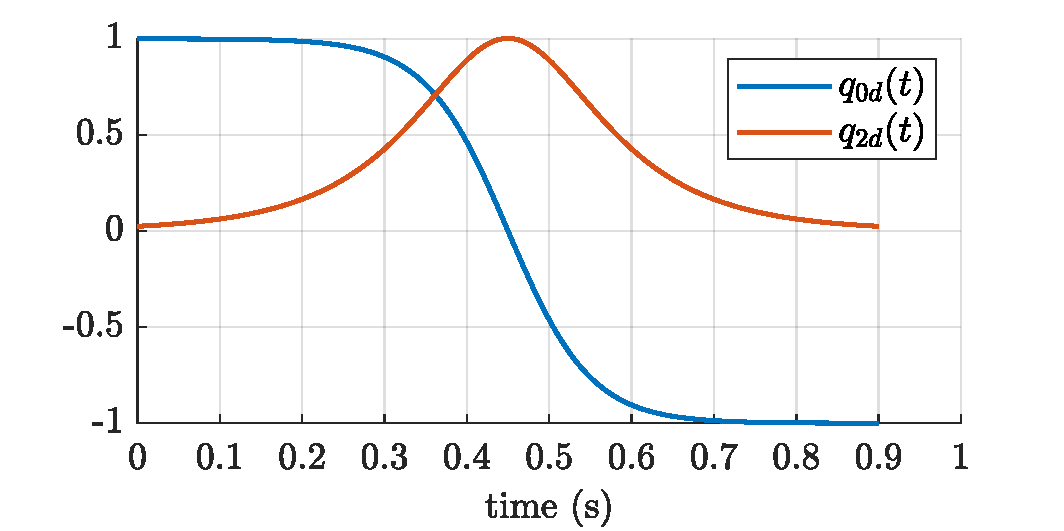
\includegraphics[width=10cm]{Fig/quat_ref.pdf}
    \caption{Attitude quaternion reference trajectory for the backflip maneuver with $\alpha=20$ 1/s, $\beta = 0.45$ s.}
    \label{fig:attref}
\end{figure}

A 360 degree turn around the pitch axis means that the scalar part of the attitude quaternion goes from 1 to -1. In the trajectory design it is important to stay within the $q_{0d}\in [-1, 1]$ range, because only unit quaternions describe rotation. We have chosen a smooth sigmoid function
\begin{equation}\label{eq:sigmoid}
    q_{0d} = \frac{2}{1+e^{-\alpha(t-\beta)}}-1
\end{equation}
to describe the scalar part of the reference attitude, where the parameters are the speed of the maneuver $\alpha$ and half of the duration of the flip $\beta$. The attitude quaternion reference trajectory is displayed in Figure \ref{fig:attref}.

The position reference need to be design considering that the rotational and translational equations of the dynamical model are coupled. The motion of the flip maneuver is within the $x-z$ plane, therefore $y_d(t) = 0$. The other two equations of \eqref{eq:geom_tran} are
\begin{subequations}\label{eq:any}
    \begin{align}
       m \ddot x & = - Fr_{13}',\\
        m \ddot{z} & = - F r_{33}' + mg,  
    \end{align}
\end{subequations}
where $r_{ij}'$ is the element of the rotation matrix $R$ in the $i$th row and $j$th coloumn. However, assuming that the attitude tracking converges fast enough to the reference, we can substitute the reference rotation matrix in \eqref{eq:any}, resulting in the translational state space representation
%\begin{subequations}
    \begin{align}\label{eq:linsys}
    \frac{\mathrm{d}}{\mathrm{d}t} \underbrace{\begin{bmatrix} x \\ \dot x \\ \tilde z \\ \dot{\tilde{z}}\end{bmatrix}}_{\mathbf{x}} = \underbrace{\begin{bmatrix} 0 & 1 & 0 & 0 \\ 0 & 0 & 0 & 0 \\ 0 & 0 & 0 & 1 \\ 0 & 0 & 0 & 0 \end{bmatrix}}_{\mathbf{A}} \begin{bmatrix} x \\ \dot x \\ \tilde z \\ \dot{\tilde{z}} \end{bmatrix} + \underbrace{\begin{bmatrix} 0 \\ r_{13}/m \\ 0 \\ r_{33}/m \end{bmatrix}}_{\mathbf{B}}  F
      % m \ddot x & = - Fr_{13},\\
      %  m \ddot{z} & = - F r_{33} + mg,  
    \end{align}
%\end{subequations}
where $r_{ij}$ are the corresponding elements of the reference rotation matrix $R_d$, converted from the reference quaternion, and $\mathbf A, \mathbf B$ are the state space matrices. As the equations are decoupled, the effect of gravity can be added to the $z$ position after a simulation, thus in the equation $\tilde{z}$ denotes the modified state. Notice that \eqref{eq:linsys} is a linear state space representation with the thrust force $F$ as the only control input. With discretizing the system, a quadratic programming problem can be formulated to a finite horizon, similarly to model predictive control.

The discrete state space model can be calculated as \cite{linearsys}
\begin{align}
    & \mathbf x_{k+1} = \mathbf A_d \mathbf x_k + \mathbf B_d u_k,\\
    & \begin{bmatrix} {\mathbf A_{d}} & {\mathbf B_{d}} \\ {\mathbf 0} & {\mathbf I} \end{bmatrix}= \mathrm{exp}\left({{\begin{bmatrix} \mathbf{A} & {\mathbf B} \\ \mathbf{0} & \mathbf{0} \end{bmatrix}}T_s}\right),
\end{align}
where $\mathbf A_d, \mathbf B_d$ are the discrete state space matrices, $\mathbf 0$ and $\mathbf I$ denote the zero and identity matrices with suitable size, $T_s$ is the sampling time and the exp$(\cdot)$ operator is the matrix exponent. The input of the model is the collective thrust of the propellers, $u_k=F_k$.

For a fixed duration of the maneuver with $N$ discrete time steps, the optimization problem is formulated as
\begin{subequations}\label{eq:quadprog}
    \begin{align}
        &\min_u \sum_{k=1}^N \left[ \left(\mathbf x_k-\mathbf x_{d,k}\right)^\top \mathbf Q_k  \left(\mathbf x_k-\mathbf x_{d,k}\right) + u_k^\top R_k u_k\right], \text{ s.t.}\\
        &\mathbf x_{k+1} = \mathbf A_d \mathbf x_k +\mathbf B_d u_k,\\
        &\{ \mathbf x_{k}\}_{k=1}^N \in \mathcal{X},\\
        &\{u_{k}\}_{k=0}^N \in \mathcal{U},
    \end{align}
\end{subequations}
where $\mathbf Q_k\in \mathbb{R}^{4\times 4}$ and $R_k \in\mathbb{R}$ are weight matrices, and $\mathcal{X}, \mathcal{U}$ are the sets of constraints for the states and the control input, respectively. In this case, we can specify linear constraints for the states, for example $x\in[x_-,x_+], z\in[z_-, z_+]$, and also linear constraint for the control input, namely
    \begin{align}
        \frac{\norm{\tau_k}}{l} \leq u_k = F_k \leq F_\mathrm{max}-\frac{\norm{\tau_k}}{l},
    \end{align}
where $\tau_k$ is the vector of the three torques around the three body axes, out of which $\tau_x=\tau_z=0$ normally during the flip, $l$ is the distance of the quadcopter center of mass and the propellers projected to the $x-z$ plane, and $F_{max}$ is the maximal collective thrust of the rotors. The torque control input $\tau_k$ is calculated from the reference attitude $R_d$ based on \eqref{eq:geomtau} assuming that the orientation and angular velocity errors are zero.

The only objective of the trajectory design is to minimize the final position error of the quadcopter and keep the position within a specified range, therefore the weight matrices are $R_k = 0, \mathbf Q_k=0$ for $k=1\dots N$, except for the weight of the final state that is
\begin{equation}
\mathbf Q_N = \begin{bmatrix} 1 & 0 & 0 & 0 \\ 0 & 0 & 0 & 0 \\ 0 & 0 & 1 & 0 \\ 0 & 0 & 0 & 0 \end{bmatrix}.
\end{equation}
As all the other weights are zero, it is only required to specify a final state position reference that is defined as
\begin{equation}
    \mathbf x_{d,N} = \begin{bmatrix} x_{d,N} \\ \dot{x}_{d,N} \\ {\tilde{z}}_{d,N} \\ \dot{\tilde{z}}_{d,N} \end{bmatrix} = \begin{bmatrix} 0 \\ 0 \\ \frac{1}{2}g(T_s N)^2 \\ 0 \end{bmatrix}.
\end{equation}

The solution of a quadratic optimization program with linear constraints is a built-in feature of most engineering programming languages, for example the \verb+quadprog+ function in Matlab. 